\documentclass{article}

\usepackage{arxiv}

\usepackage[utf8]{inputenc}
\usepackage[T1]{fontenc}
\usepackage{url}
\usepackage{booktabs}
\usepackage{amsfonts}
\usepackage{nicefrac}
\usepackage{microtype}
\usepackage{graphicx}
\usepackage[font=small,labelfont=bf]{caption}
\usepackage{cite}
\usepackage{pdflscape}
\usepackage{listings}
\usepackage{outlines}

\title{Logs lineage and tiered segments in Apache Kafka}

\begin{document}

\section{Objectives}
The purpose of this document is to describe how tiered log segments are handled to preserve a uniform access to data.

\subsection{Data uniformity}

The targeted functional behaviour is to provide the same data to consumers regardless of the origin of these data. This \textit{uniformity} property requires to reproduce the current behaviour of Apache Kafka for which log segments are always accessed locally. Especially, the current specifications under divergence of log lineage should be preserved, and no discrepancy should be introduced in the data a consumer would expect to find with or without tiered storage.

\subsection{Log lineage divergence and remote duplication}

It is possible that a log segment which is offloaded (uploaded) to a tiered storage presents offset overlap or contains duplicated and/or divergent records with already tiered log segments (as after an unclean leader election).
Such cases will be studied thereafter and the expected behaviour described.

\section{Log lineage divergence}

One consequence of unclean leader election is a possible divergence of log lineages which can happen when leadership of a topic-partition moves to an out-of-sync replica. 

Let us consider the following illustrative example. A topic-partition is made of two replicas 1 and 2. In order to simplify, we assume a strict correspondance of log segment base and end offsets in both replicas. The cases where this cannot be assumed will be explored later in the document.

Let $S_i$ be the i-th log segment in either replica and $BO_i$ and $EO_i$ the base and end offsets of $S_i$. 

Let us assume unclean leader election is enabled. 

\begin{outline}[enumerate]
	\1 At $t_1$, replica 1 is the leader and replica 2 is out of ISR. The segment $S_i$ has been rolled over in replica 1, for which $S_{i+1}$ is the active segment. Since the ISR is reduced to the leader replica, the leader high watermark of the leader can progress and follow the log end offset. Assume there is no transactional records, so that the log stable offset corresponds to the leader high watermark, or, without loss of generality, assume the LSO points to an offset of $S_{i+1}$. The segment $S_i$ is therefore eligible for tiering. Assume the leader of replica 1 offloads successfully $S_i$. Assume that afterwards, that segment is locally deleted following the configured log's retention policy.
	\1  At $t_2$, replica 1 become offline and replica 2 becomes the only online replica of the topic-partition.
	\1  At $t_3$, replica 2 uncleanly acquires the leadership of the topic-partition and the leader epoch is incremented from $k$ to $k + 1$.
	\1  At $t_4$, replica 1 is online and becomes a follower of replica 2. It starts replicating with a fetch offset set to its high watermark, the last offset of segment $S_{i+1}$. This offset is ahead of the latest offset of replica 2, and the first replication fetch request fails (index out of bound). The follower then fetches the LEO for generation $k+1$ or $LEO_{k+1}$. It truncates its local segment to the returned offset.
	\2 Without tiered storage - segment $S_i$ was deleted from the local storage and the local log start offset is ahead of $LEO_{k+1}$. Therefore, the follower truncates fully (i.e. delete all current segments) and creates a new segment with a start offset equal to $LEO_{k+1}$, and start fetching from that offset.
	\2 With tiered storage - a segment which includes $LEO_{k+1}$ in its offset range is present in the tiered storage. 
	\3 This segment can be ignored and the behaviour would be the same as without tiered storage.
	\3 The segment can be onloaded and promoted back to an active segment, truncated to $LEO_{k+1}$, and replication would start from that offset. Some records of replica 1 diverge from replica 2.
	\1 Replica 2 ingests more records. Segment $S_i$ is rolled over. Because it is part of the log lineage at generation $k+1$. and offloaded to the tiered storage.
	

	
\end{outline}

\begin{center}
	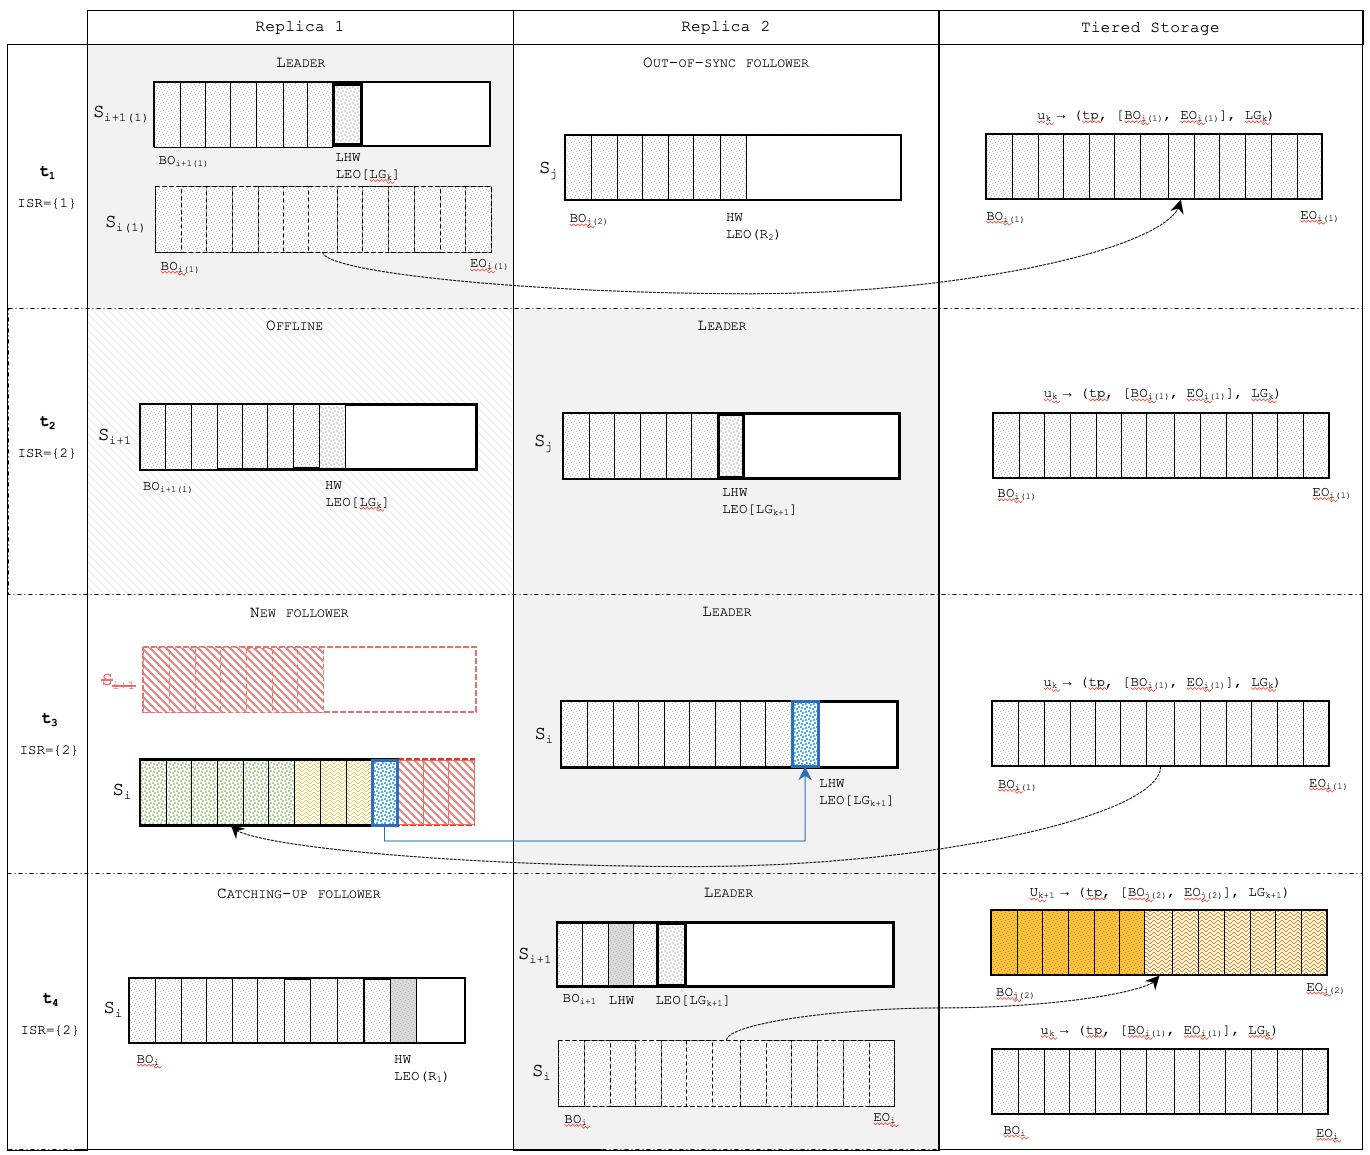
\includegraphics[scale=0.45]{unclean1.png}
	\captionof{figure}{}
\end{center}



\end{document}
